\documentclass[usletter,11pt]{article}


\usepackage{graphicx}
\usepackage[table]{xcolor}
\usepackage{booktabs}
\usepackage{colortbl}
\usepackage{newcent}
\usepackage{sectsty}
\usepackage{fancyhdr}
\pagestyle{fancy}
\usepackage{calc}
\usepackage{listings}
\usepackage{array}
\usepackage{tikz}
\usepackage{amsmath}
\renewcommand{\headrule}{{\color{brightOrange}%
  \hrule width\headwidth height\headrulewidth \vskip-\headrulewidth}}
\renewcommand{\footrule}{{\color{brightOrange}%
  \hrule width\headwidth height\headrulewidth \vskip-\headrulewidth}}

\newcommand{\referee}[1]{
\begin{center}
\begin{tikzpicture}
\node[fill=paleOrange, rounded corners=0.3cm]{
%\hspace{0.1cm}
 \parbox{\textwidth}{
  \vspace{0.15cm}
#1
  \vspace{0.15cm}
 }
%\hspace{0.1cm}
};
\end{tikzpicture}
\end{center}
}

\newcommand{\member}[2]
{ \noindent
{ \color{softBlue}  #1 - } #2
\vspace{0.2cm}
}

\fancyheadoffset[LE,RO]{\marginparwidth}
\fancyfootoffset[LE,RO]{\marginparwidth}
\fancyhead{} % clear all header fields
\fancyhead[LE,RO]{\color{softBlue}  \sffamily The CXI File Format for Coherent X-ray Imaging}
%\fancyhead[R]{\color{softBlue} \thepage \vspace{-0.08cm}}


\fancyfoot{} % clear all header fields
\fancyfoot[L]{\vspace{0.1cm}
\includegraphics[width=0.35\textwidth]{cxidb_logo_header2.pdf}}
\fancyfoot[R]{\vspace{1.0cm}\color{softBlue}\thepage}
%\renewcommand{\footrulewidth}{1pt}


\usepackage{setspace}

\definecolor{tableBlue}{RGB}{231,244,249}
\definecolor{linkBlue}{RGB}{32,75,165}
\definecolor{brightOrange}{RGB}{210,131,37}
\definecolor{ironGrey}{RGB}{64,73,78}
\definecolor{steelGrey}{RGB}{70,91,102}
\definecolor{cloudyGrey}{RGB}{104,132,150}
\definecolor{lightGrey}{RGB}{184,198,206}
\definecolor{softBlue}{RGB}{29,97,134}
\definecolor{paleOrange2}{RGB}{233,185,128}
\definecolor{paleOrange}{RGB}{248,219,167}
\definecolor{typeGreen}{RGB}{19,101,106}

\usepackage{caption}
\DeclareCaptionFont{white}{\color{white}}
\DeclareCaptionFont{softBlue}{\color{softBlue}}
\DeclareCaptionFormat{listing}{\colorbox{softBlue}{\parbox{\textwidth}{\hspace{15pt}#1#2#3}}}
\captionsetup[lstlisting]{format=listing,labelfont=white,textfont=white,
  singlelinecheck=false, margin=0pt, font={sf,footnotesize}}
\captionsetup[figure]{labelfont={softBlue,bf},
 singlelinecheck=false, margin=0pt, font={small}}
\captionsetup[table]{labelfont={softBlue,bf},
 singlelinecheck=false, margin=0pt, font={footnotesize},justification=centering}



\newcommand{\HRule}{{\color{brightOrange} \rule{\linewidth}{0.5mm}}}

\allsectionsfont{\color{softBlue} \usefont{OT1}{pag}{b}{n}\selectfont}

\usepackage[linkcolor=softBlue,colorlinks=true,urlcolor=softBlue]{hyperref}
%\usepackage[table,usenames,dvipsnames]{color}


\begin{document}


\begin{center}
\vspace*{2.5cm}

\includegraphics[width=0.8\textwidth]{cxidb_logo_large.pdf}\\[2.0cm]

\HRule \\[0.6cm]
\begin{spacing}{2.0}
{\color{softBlue} \Huge \sffamily The CXI File Format for Coherent
 X-ray Imaging}\\[0.2cm]
\end{spacing}
\HRule \\[1.0cm]
{\Large \color{softBlue} \sffamily Draft Version 1.1}\\[4.5cm]

{\Large \color{softBlue} \sffamily Filipe R. N. C. Maia}\\[0.3cm]
{\Large \color{softBlue} \sffamily \today}
\thispagestyle{empty}
\end{center}

\pagebreak

\thispagestyle{fancy}
\pagenumbering{Roman}

\tableofcontents

\pagebreak

\pagenumbering{arabic}


\setcounter{page}{1}

\section{Introduction}
The CXI file format was created as common format for all the data in the Coherent X-ray Imaging Data Bank (CXIDB).
Naturally its scope is all experimental data collected during Coherent X-ray Imaging experiments as well as all data generated during the analysis of the experimental data.

\subsection{Goals}
The CXI file format aims to create a data format with the following requirements:
\begin{enumerate}
\item{Simple - both writing and reading should me made simple.}
\item{Flexible - users should be able to easily extend it.}
\item{Fast - it should be efficient so as not to become a bottleneck.}
\item{Extendable - new features should be easily added without breaking compatibility with previous versions.}
\item{Unambiguous - it should be possible to interpret the files without using external information.}
\item{Compatible - the format should be as compatible as possible with existing formats}
\end{enumerate}

These are hard and often contradicting requirements (e.g. simple and unambiguous). When such conflicts occur the highest ranked goal is often prefered (e.g. simple). 

\section{The Design of the CXI} 

\subsection{HDF5}

The HDF5 format is the basis of CXI format. CXI is not really a completely new file format but simply a set of rules designed to create HDF5 files with a common structure and to allow a uniform and consistent interpretation of such files.

HDF5 was chosen as the basis because it is a widely used high
performance scientific data format which many programs can already, at
least partially,  read and write. It also brings with it the almost
automatical fulfilment of requirements 2, 3 and 4. HDF5 version 1.8 or
higher is required as previous versions don't support all features
required by CXI.

\subsection{NeXus}
Another important influence in the design of CXI is the NeXus file format for neutron, x-ray and muon science.
As CXI, NeXus is also based on HDF5 (although it can use others basis formats such as XML) and shares many of the goals of CXI, with one important exception - it is {\em not} a simple format. All NeXus file require attributes in HDF5 files and using many existing programs it is laborious and hard, if not outright impossible, to create such attributes. The large scope of NeXus also results in files that can be complex to read and interpret.

NeXus classes are the fundamental pieces that make up NeXus files. The documentation for the classes can be found in \url{http://download.nexusformat.org/doc/html/ClassDefinitions.html}. Each class has a set of members which can either be data fields with well defined members (e.g. the {\tt data} field of the \hyperref[table:data]{\tt NXdata} class), or they can be other classes in which case the name is arbitrary. Each NeXus class corresponds to an HDF5 group with one or more attributes (class name, units, long name, etc...) and each class data field corresponds to an HDF5 dataset. 
\subsection{CXI}

The approach used in CXI is to use HDF5 as basis format and adopt a small set of rules derived from the NeXus format with some additional restraints which should make the format simpler to write and interpret. This allows us to relax the format, making it simple for new users, while still retaining enough information to reconstruct an NeXus compile file if necessary.

Below are the main rules used in CXI files:
\begin{itemize}
\item{Groups representing NeXus classes should be named like the class
    with the {\tt NX} prefix removed and with {\tt \_$N$} added where
    $N$ are consecutive positive integers starting at 1
    (e.g. {\tt entry\_1} represents the first
    \hyperref[table:entry]{\tt NXentry}).}
\item{NeXus class fields should be used as much as possible.}
\item{Each data field must have default units.}
\item{Non default units are defined using the {\tt units} attribute of relevant dataset, just like in NeXus.} 
\end{itemize}

\section{CXI by example}
\subsection{A minimal CXI file}
Figure \ref{fig:minimal} shows a diagram a minimal CXI file. Each measurement (which is usually an exposure/shot) in a CXI file is stored inside a group named {\tt entry\_$N$} where $N$ is a positive integer. The first such entry should be named {\tt entry\_1} the second {\tt entry\_2} and so on. Each entry is a member of the NXentry class in NeXus language.

\begin{figure}[h!]
\centering
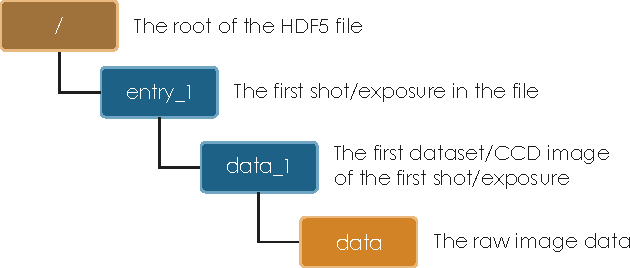
\includegraphics[width=0.8\textwidth]{minimal_cxi.pdf}
\caption{Diagram of a minimal CXI file with a single image.}
\label{fig:minimal}
\end{figure}

The arrangements of the HDF5 groups is similar to that in a NeXus file. The main difference is that in a NeXus file entries are not identified by name but by the {\tt NX\_class} attribute which is set to \hyperref[table:entry]{\tt NXentry}. In a CXI file we restrict the possible names of a measurement group to only {\tt entry\_$N$} simplifying things by not requiring the attribute. Yet a simple post processing program could take a CXI file an easily convert it into a NeXus file by adding the required attributes. This is the {\em main design idea} of the CXI format and we will see examples of it in many places.

Each entry can have one or more data groups. In this case we only had one detector so we only have one data group named {\tt data\_1}. The raw data is stored in the {\tt data} field of the {\tt data\_1} group. As no units are specified the data is assumed to be in ``counts'' (see \ref{units}). Also no experimental data about the experimental conditions is stored.

\subsection{A typical raw data CXI file}

\begin{figure}[h!]
\centering
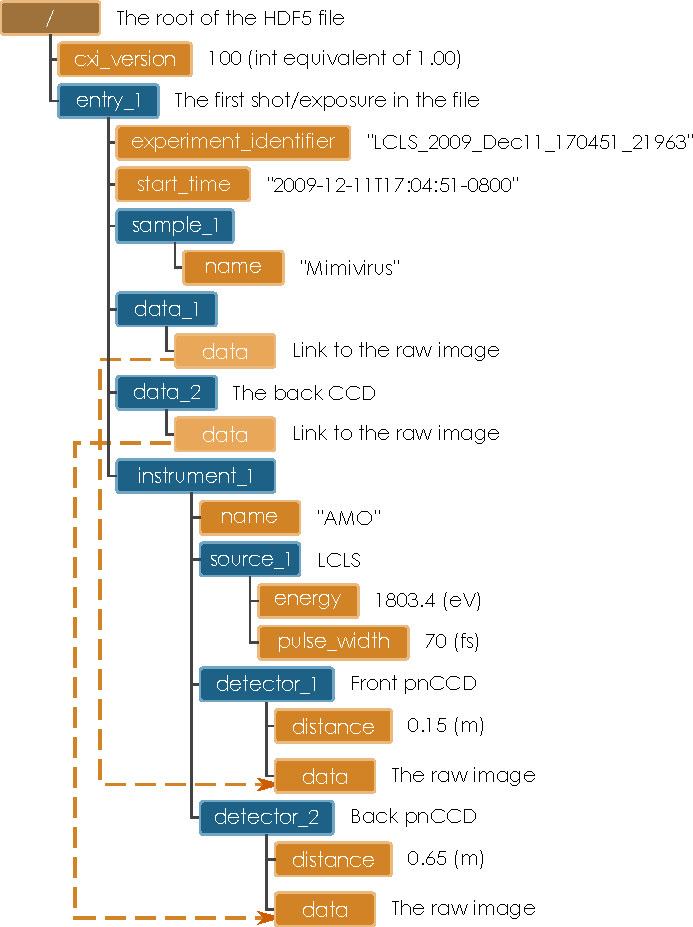
\includegraphics[width=0.7\textwidth]{lcls_camp_cxi.pdf}
\caption{Diagram of a typical CXI file for storing raw data from a single shot.}
\label{fig:lcls_camp_raw}
\end{figure}

\clearpage
\section{NeXus compatibility}
One of the most appealing features of the CXI format is that while it is relatively simple it can still be unambiguously converted to follow the NeXus format.

Figure \ref{fig:lcls_camp_raw_nexus} shows the convertion of the example in figure \ref{fig:lcls_camp_raw} to the NeXus format. Note that the only change are the addition of several attributes that are necessary for NeXus. This means that CXI files can be easily converted to NeXus, then edited using NeXus based tools if necessary, and then read back using a CXI based tool.

\begin{figure}[h!]
\centering
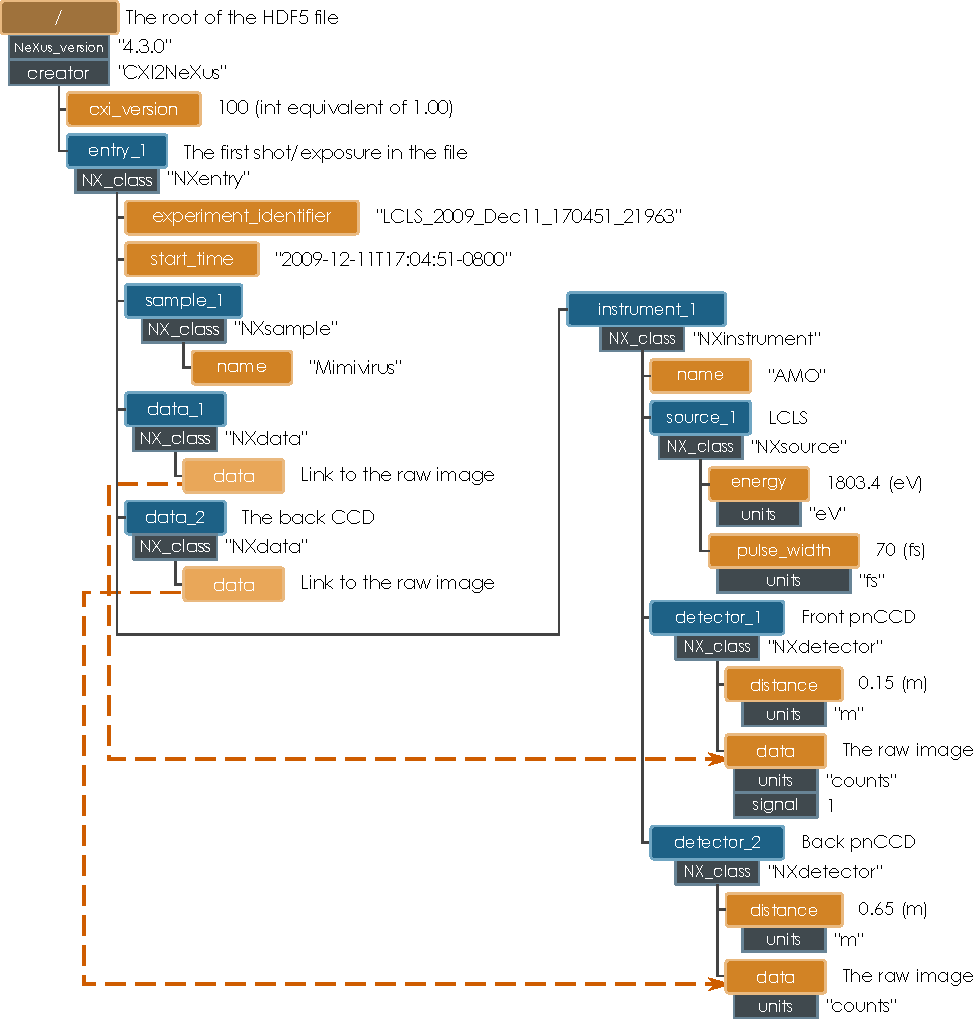
\includegraphics[width=0.9\textwidth]{lcls_camp_cxi_nexus.pdf}
\caption{Diagram of a NeXus compatible CXI file for storing raw data from a single shot.}
\label{fig:lcls_camp_raw_nexus}
\end{figure}


\clearpage
\section{Datatypes}

HDF5 covers a large variety of native datatypes including integers,
floating point numbers and character string(includng UTF-8
support). It also takes care of the conversion of datatypes when
reading and writing files (eliminating endianess problems for
example). 

Most of the data should be saved in the same format as it was
created/aquired. For example CCD images acquired as 16 bit integers
should be saved using the {\tt H5T\_NATIVE\_SHORT} HDF5 Type.

\subsection{Complex Numbers}

A notable omission of the HDF5 1.8 standard, in which this format is
based on, is the lack of a standard way to store complex numbers.

The CXI convention for storing complex numbers is to use a compound data
type with two elements named {\tt r} and {\tt i}. The real part of the
number should obviously be saved in the element named {\tt r} and the imaginary
part in the one named {\tt i}. This follows the convention adopted by
PyTables as well as h5py.

Below you can see a C99 code snippet showing how to create a CXI compatible HDF5
compound type for double complex numbers.

\lstset{
emph={[2]complex}, 
 emph={[3]H5Tcreate}, 
 emph={[4]H5Tinsert}, 
emph={[5]sizeof}, 
 emph={[6]i}, 
 emph={[7]r},
 emph={[8]double}, 
 emph={[9]hid_t}, 
caption={Creating a double complex type},
  label=lst:complex_type,
  frame=b,
  basicstyle=\footnotesize\ttfamily,
  breaklines=true,
  stringstyle=\color{brightOrange}\ttfamily\bfseries,
  xleftmargin=17pt,
  framexleftmargin=17pt,
  framexrightmargin=5pt,
  framexbottommargin=4pt,
  numbersep=5pt,
  extendedchars=true,
  showstringspaces=false, 
  keywordstyle=\color{softBlue}\ttfamily,
  emphstyle=\color{softBlue}\ttfamily,
  emphstyle=[2]\color{typeGreen}\ttfamily,
  emphstyle=[3]\color{softBlue}\bfseries\ttfamily,
  emphstyle=[4]\color{softBlue}\bfseries\ttfamily,
  emphstyle=[5]\color{typeGreen}\bfseries\ttfamily,
  emphstyle=[6]\color{brightOrange}\bfseries\ttfamily,
  emphstyle=[7]\color{brightOrange}\bfseries\ttfamily,
  emphstyle=[8]\color{typeGreen}\ttfamily,
  emphstyle=[9]\color{typeGreen}\ttfamily
}
\begin{lstlisting}
hid_t complex_id = H5Tcreate(H5T_COMPOUND, 
                            sizeof(double complex));
H5Tinsert(complex_id, "r", 0, H5T_NATIVE_DOUBLE);
H5Tinsert(complex_id, "i", sizeof(double), H5T_NATIVE_DOUBLE);
\end{lstlisting}

\clearpage
\section{Default units for CXI entries}
\label{units}

The default units for all CXI entries are SI base units (see table
\ref{table:SI}) with {\em no exceptions}.

\begin{table}[h!]\sffamily \small
\caption{SI (and common derived) base units for different quantities}
\label{table:SI}
\begin{center}
\centering
\rowcolors{1}{white}{tableBlue}
\begin{tabular}{p{4.5cm} p{4.5cm}  p{2.5cm}}
\doublerulesepcolor{tableBlue}
\toprule
\bfseries Quantity   & \bfseries Units & \bfseries Abbreviation \\
\doublerulesepcolor{tableBlue}
\midrule
length & meter & m \\
mass & kilogram & kg \\
time & second & s \\
electric current & ampere & A \\
temperature & kelvin & K \\
amount of substance & mole & mol \\
luminous intensity & candela & cd \\
\midrule
frequency & hertz & Hz \\
force & newton & N \\
pressure & pascal & Pa \\
energy & joule & J \\
power & watt & W \\
electric potential & volt & V \\
capacitance & farad & F \\
electric resistance & ohm & $\Omega$ \\
absorbed dose & gray & Gy \\
area & square meter & m$^2$ \\
volume & cubic meter & m$^3$ \\
\bottomrule
\end{tabular}
\end{center}
\end{table}


\subsection{Angles}
Angles are always defined in degrees {\em not} in radians.

\subsection{Dates} 
Dates are always specified according to the \href{http://www.w3.org/TR/NOTE-datetime}{ISO 8601}.  This means for example ``1996-07-31T21:15:22+0600''.
Note the ``T'' separating the data from the time and the ``+0600'' timezone specification.

All of these are mandatory.
They derive from the use of ISO 8601 in NeXus. This way compatibility is ensured.

\section{Memory Layout}
All multidimensional arrays must be stored with the fastest changing
dimension being the last dimension, and the slowest changing dimension
being the first dimension, also known as row major. This is defined in
the HDF5 standard.

\section{Geometry}
\subsection{Coordinate System}
CXI uses the same coordinate system as NeXus which itslef is 
based on the McStas coordinate system (NeXus User Manual section
2.2.1). 

The CXI coordinate system is a right handed system. The z axis
parallel to the X-ray beam, with the positive z direction pointing away
from the light source, in the downstream direction. This is the {\em
  opposite} of the definition of the International Tables for
Crystallography, volume G. The y axis is vertical with the positive
direction pointing up, while the x axis is horizontal completing the
right handed system (see Fig. \ref{fig:cxi_coord_system}).

The origin of the CXI coordinate system is defined by the point where the X-ray
beam meets the sample.

\begin{figure}[h!]
\centering
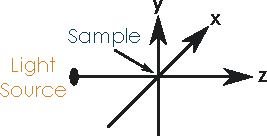
\includegraphics[width=0.6\textwidth]{coord_system.pdf}
\caption{The coordinate system used by CXI. The intersection of the
X-ray beam with the sample define the  origin of the system. The z
axis is parallel to the beam and
points downstream.}
\label{fig:cxi_coord_system}
\end{figure}

\subsection{The local coordinate system of objects}
\label{originOfObjects}

For many detectors their location and orientation is crucial to
interpret results. 

Translations and rotations are used to define
the absolute position of each object. But to be able to apply these
transformations we need to know what is the origin of the local
coordinate system of each object.

Unless otherwise specified the origin should be assumed to be the
geometrical center of the object in question. The default orientation
of the object should have the longest axis of the object aligned with
the x axis, the second longest with the y axis and the shortest with
the z axis.

\subsubsection{The orientation of pixel detectors}
\label{ccd_orientation}

The location and orientation of pixel detectors is particularly important for
diffraction experiments.

For convenience specific rules have been defined for the coordinate
system of pixel detectors. Instead of defining a local origin plus a
default orientation the detectors are defined in absolute terms by a
corner\_position plus a set of basis\_vectors.

The corner\_position should contain the x, y and z coordinates of the corner of
the first data element which corresponds to the corner of the
detector. The corner\_position must always be defined.
  
Figure \ref{fig:detector_coordinates} gives an example.

\begin{figure}[h!]
  \centering
  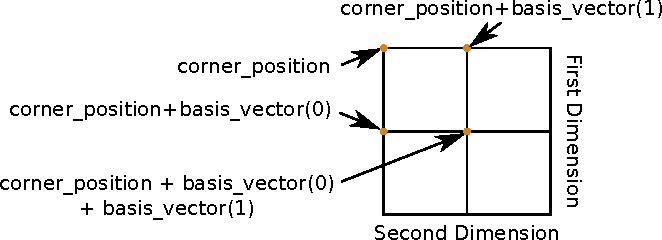
\includegraphics[width=0.7\textwidth]{detector_coordinates.pdf}
  \caption{The coordinates of the four corners of the first pixel in a
    pixel detector.}
  \label{fig:detector_coordinates}
\end{figure}

The basis\_vectors are a matrix containing a set of 3D vectors from the
center of the first element to the center of the second element
for each dimension of the detector. The number of rows of the matrix
(first dimension) is equal to the number of dimensions of data and the
number of columns (second dimension) is equal to 3 (the x, y and z position in 3D space).

The first row then defines the relative distance between the first two
pixels in the first dimension (e.g. position of (1,0) - position of
(0,0) for a 2D array),
and the second row elements do the same along the second dimension (e.g. position of
(0,1) - position of (0,0) for a 2D array).

If no basis\_vectors are specified they are assumed to be:
\[
 \begin{bmatrix}
  0 & -y\_pixel\_size & 0 \\
  -x\_pixel\_size & 0 & 0 
\end{bmatrix}
\]

This results in the first dimension parallel to the y axis and the second to the x
axis. This convention should be used as much as possible as many
programs will assume it when displaying data. If more dimensions are
required it's strongly encouraged to make the last two dimension
correspond to the y and x axis.

\begin{figure}[h!]
\centering
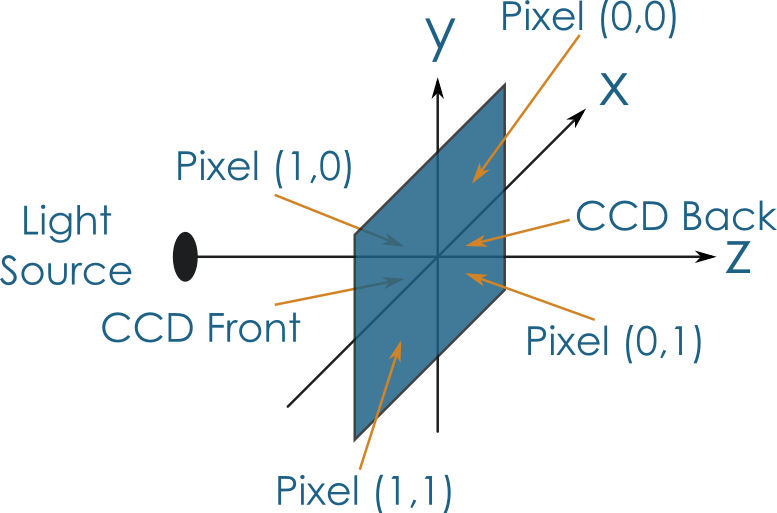
\includegraphics[width=\textwidth]{detector_coord_system.png}
\caption{Pixel locations for a pixel detector with no basis\_vectors
  defined or rotation applied and with a corner\_position of (pixel
  width, pixel height, detector distance).}
\label{fig:detector_coord_system}
\end{figure}

\clearpage
\appendix
\section{More CXI file examples}

\subsection{CXI file from a ptychography experiment}

\begin{figure}[h!]
\centering
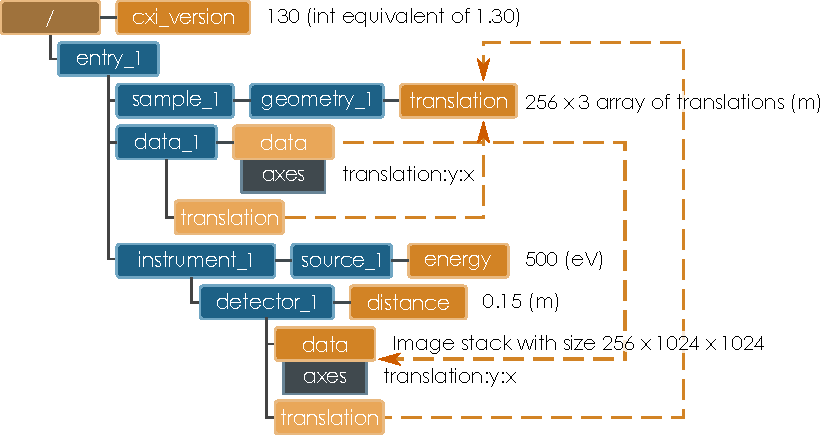
\includegraphics[width=0.9\textwidth]{ptychography_cxi.pdf}
\caption{Diagram of a CXI file with 256 diffraction images from a ptychography experiment.}
\label{fig:ptychography_cxi}
\end{figure}


\clearpage
\subsection{CXI file after initial analysis of a diffraction image}

\begin{figure}[h!]
\centering
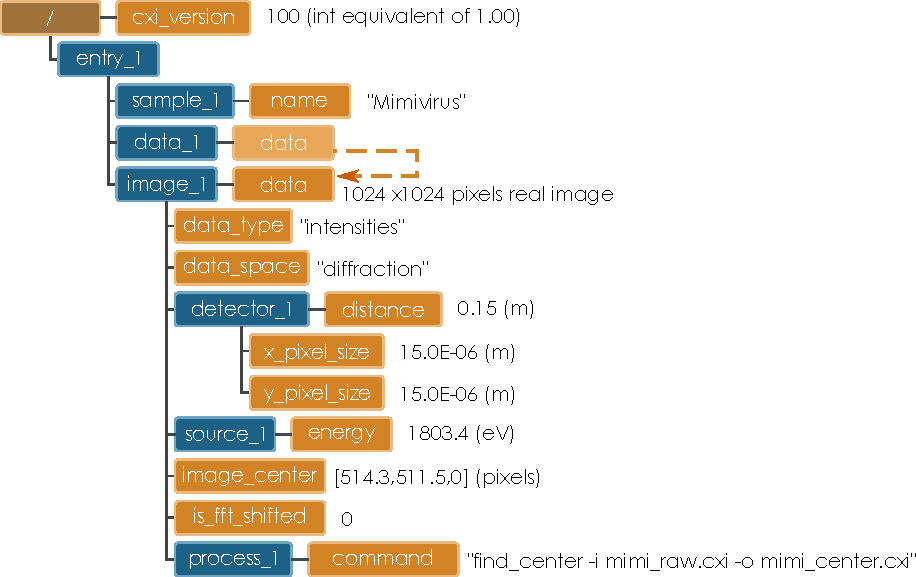
\includegraphics[width=\textwidth]{analysed_image.pdf}
\caption{Diagram of a CXI file of an analysed image from a single
particle diffraction experiment.}
\label{fig:analysed_image}
\end{figure}


\clearpage
\subsection{CXI file of a phased 3D image}

\begin{figure}[h!]
\centering
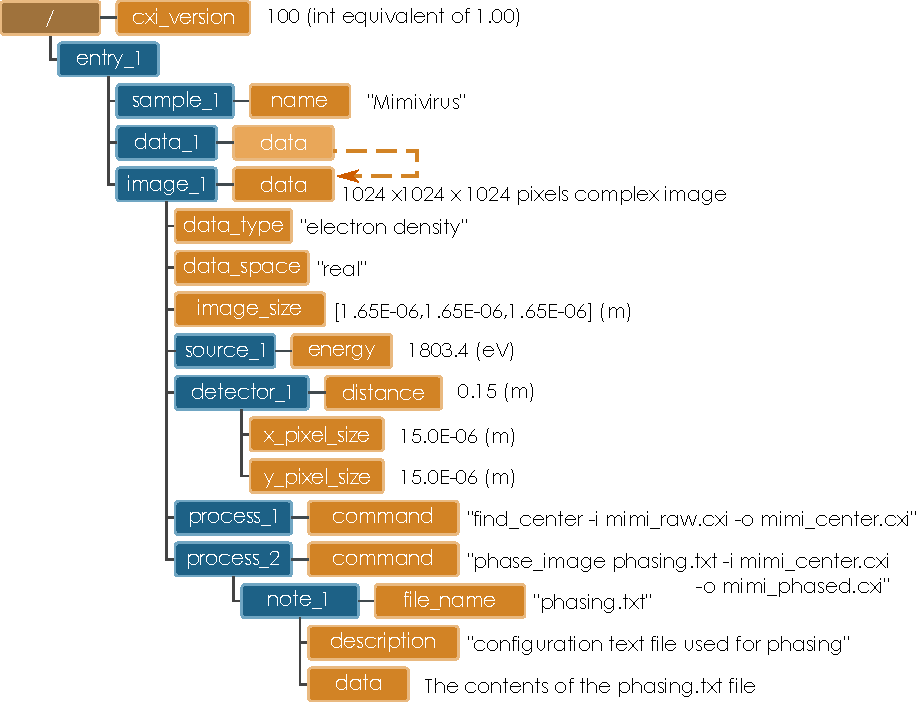
\includegraphics[width=\textwidth]{phased_image.pdf}
\caption{Diagram of a CXI file of a phased 3D image from a single
particle diffraction experiment.}
\label{fig:phased_image}
\end{figure}

\clearpage

\section{CXI entries reference}

\subsection{Top level (root)}
\label{table:top}

This node represents the top level of the HDF5 file and holds some
general information about the file as well as number of entries.

\begin{table}[h!]\sffamily
\footnotesize
\caption{CXI top level entries}

\rowcolors{1}{white}{tableBlue}
\begin{tabular}{p{4.5cm} p{4.5cm}  p{2.5cm}}
%\begin{tabular}{p{4.5cm} p{3cm}  p{4cm}}
%\begin{tabular}{lllp{6cm}}
\toprule
\bfseries Member     & \bfseries Type & \bfseries Quantity \\
\midrule

cxi\_version & int & version  \\
entry\_$N$ &  \hyperref[table:entry]{Entry class} & \\
number\_of\_entries & int & unitless \\
\bottomrule
\end{tabular}
\end{table}

\member{cxi\_version}{CXI format version times 100. Version 1.00 would
  be represented by 100 and 1.5 by 150.}

\member{entry\_$N$}{The measurements recoded in this file.}

\member{number\_of\_entries}{Total number of entries in the file.}

\subsection{Attenuator}
\label{table:attenuator}

This class describes a beamline attenuator used during data collection.

\begin{table}[h!]\sffamily \footnotesize
\caption{Attenuator class members}

\rowcolors{1}{white}{tableBlue}
\begin{tabular}{p{4.5cm} p{4.5cm}  p{2.5cm}}
%\begin{tabular}{p{4.5cm} p{3cm}  p{4cm}}
\toprule
\bfseries Member     & \bfseries Type & \bfseries Quantity \\
\midrule
distance & float & length \\
thickness & float & length \\
attenuator\_transmission & float & unitless \\ 
type & string & text \\
\bottomrule
\end{tabular}
\end{table}

\member{distance}{Distance from sample.}

\member{thickness}{Thickness of attenuator along beam direction.}

\member{attenuator\_transmission}{The nominal amount of the beam that
gets through (transmitted intensity)/(incident intensity).}

\member{type}{Type or composition of attenuator.}

\subsection{Data}
\label{table:data}

This class is a general placeholder for the most important information
in each Entry class. It is mandatory that there is at least one Data
class in each Entry class. Most data analysis and plotting programs
will primarily focus in this class.

\begin{table}[h!]\sffamily \footnotesize
\caption{Data class members}

\rowcolors{1}{white}{tableBlue}
\begin{tabular}{p{4.5cm} p{4.5cm}  p{2.5cm} }
\toprule
\bfseries Member     & \bfseries Type & \bfseries Quantity \\
\midrule
data  & float/complex array & variable  \\
errors  & float/complex array & variable \\
\bottomrule
\end{tabular}
\end{table}

\member{data}{Most important data values}

\member{errors}{Standard deviations of data values}

\subsection{Detector}
\label{table:detector}

This class holds information about one of the detectors used during
the experiment. Raw data recorded by a detector as well as its position
and geometry should be stored in this class.

\begin{table}[h!]\sffamily \footnotesize
\caption{Detector class members}

\rowcolors{1}{white}{tableBlue}
\begin{tabular}{p{4.5cm} p{4.5cm}  p{2.5cm} }
\toprule
\bfseries Member     & \bfseries Type & \bfseries Quantity \\
\midrule


basis\_vectors & float array & length \\ 
corner\_position & 3 floats & length \\
counts\_per\_joule & float & unitless \\ 
data     & float/complex array & variable  \\
data\_error & float/complex array & variable \\
data\_sum & float & variable \\
description & string & text \\
distance     & float & length\\
geometry\_1 &  \hyperref[table:geometry]{Geometry class} & \\
mask & int array & unitless \\
x\_pixel\_size & float & length  \\
y\_pixel\_size & float & length \\
\bottomrule
\end{tabular}
\end{table}

\member{basis\_vectors}{A matrix with the basis vectors of the
  detector data. For more details see \ref{ccd_orientation}.
}

\member{corner\_position}{The x, y and z coordinates of the corner of
  the first data element. For more details see \ref{ccd_orientation}.
}

\member{counts\_per\_joule}{Number of counts recorded per each joule of
  energy received by the detector. The number of incident photons can
  then be calculated by:
\begin{equation*}
\text{number of photons} = \frac{\text{source energy} \times \text{data counts}}{\text{counts per joule}}
\end{equation*}
}

\member{data}{Recorded signal values.}

\member{data\_error}{The best estimate of the uncertainty in the data
value. Where possible, this should be the standard deviation, which
has the same units as the data.}

\member{data\_sum}{Sum of all the elements in the data array. This
  number is often userful as a cheap measure of data quality.}

\member{description}{name/manufacturer/model/etc. information.}

\member{distance}{Closest distance from the detector to
the sample.}

\member{geometry\_1}{Position and orientation of the center of mass of
  the detector. This should only be specified for non pixel
  detectors. For pixel detectors use basis\_vectors and
  corner\_position.}

\member{mask}{Not all the pixels in a detector might have the same
  value. This 32bit mask makes it possible to distinguish different
  kinds of pixels.

The following list defines the meaning of each
bit when is it set, as well as the names of constants, defined in {\tt
cxi.h}, useful for
checkings their values:

\begin{table}[h!]\footnotesize
\caption{Definition of each bit in the mask}
\begin{tabular*}{\textwidth}{@{\extracolsep{\fill}} l p{5.5cm} l}
\toprule
\sf \bfseries Bit & \sf \bfseries Meaning & \sf \bfseries Constant \\
\midrule
\tt \bfseries 0x00000001 & \sf If set the pixel is valid & \tt
CXI\_PIXEL\_IS\_VALID\\
\tt \bfseries 0x00000002 & \sf If set the pixel is saturated & \tt
CXI\_PIXEL\_IS\_SATURATED\\
\tt \bfseries 0x00000004 & \sf If set the pixel is hot & \tt CXI\_PIXEL\_IS\_HOT\\
\tt \bfseries 0x00000008 & \sf If set the pixel is dead & \tt
CXI\_PIXEL\_IS\_DEAD\\
\tt \bfseries 0x00000010 & \sf If set the pixel is under a shadow &
\tt CXI\_PIXEL\_IS\_SHADOWED\\
\tt \bfseries 0x00000020 & \sf If set the pixel is iluminated by
parasitic light &
\tt CXI\_PIXEL\_IS\_PARASITIC\\
\tt \bfseries 0x00000040 & \sf If set the pixel signal is above the background &
\tt CXI\_PIXEL\_HAS\_SIGNAL\\
\tt \bfseries 0x00000080 & \sf If set the pixel does not exist & \tt
CXI\_PIXEL\_DOES\_NOT\_EXIST\\
\tt \bfseries 0x00000100 & \sf If set the pixel is not exposed & \tt
CXI\_PIXEL\_NOT\_EXPOSED\\
\bottomrule
\end{tabular*}
\end{table}

All other bits have no standard meaning and can be used for any
purpose the user sees fit. More bits will be defined as the format
evolves so users are encouranged to use the high bits to avoid collisions.
}

\member{x\_pixel\_size}{Width of each detector pixel.}

\member{y\_pixel\_size}{Height of each detector pixel.}




\subsection{Entry}
\label{table:entry}

Base CXI class which holds all other classes.

\begin{table}[h!]\sffamily \footnotesize
\caption{Entry class members}

\rowcolors{1}{white}{tableBlue}
\begin{tabular}{p{4.5cm} p{4.5cm}  p{2.5cm} }
\toprule
\bfseries Member     & \bfseries Type & \bfseries Quantity \\
\midrule
data\_$N$ & \hyperref[table:data]{Data class} & \\
end\_time  & string & text \\  
experiment\_identifier & string  & text \\
experiment\_description & string & text \\
image\_$N$ & \hyperref[table:image]{Image class} & \\
instrument\_$N$ & \hyperref[table:instrument]{Instrument class} & \\ 
program\_name & string & text \\
sample\_$N$ & \hyperref[table:sample]{Sample class} &  \\
start\_time  & string & text  \\ 
title & string & text \\
\bottomrule
\end{tabular}
\end{table}


\member{data\_$N$}{Main data collected.}

\member{end\_time}{Ending time of measurement.}

\member{experiment\_identifier}{Unique identifier for the experiment,
defined by the facility, possibly linked to the proposals.}

\member{experiment\_description}{Description of the experiment.}

\member{image\_$N$}{Processed images.}

\member{instrument\_$N$}{Instrument used.}

\member{program\_name}{Name of program used to generate this file.}

\member{sample\_$N$}{Sample used.}

\member{start\_time}{Starting time of measurement.}

\member{title}{Extended title for entry}

\subsection{Geometry}
\label{table:geometry}

This class holds the general position and orientation of a component.

\begin{table}[h!]\sffamily \footnotesize
\caption{Geometry class members}

\rowcolors{1}{white}{tableBlue}
\begin{tabular}{p{4.5cm} p{4.5cm}  p{2.5cm} }
\toprule
\bfseries Member     & \bfseries Type & \bfseries Quantity \\
\midrule

orientation\_1 & \hyperref[table:orientation]{Orientation class} & \\
translation\_1 & \hyperref[table:translation]{Translation class} &  \\

\bottomrule
\end{tabular}
\end{table}

\member{orientation\_1}{The rotation of the object with respect to the
  coordinate system.}

\member{translation\_1}{The position of the object with respect to the
origin.}

Only one orientation and one translation is permitted in each geometry
class.

The position of the origin of the object should be explicitly defined for each
object. If it is not defined it should be assumed to be the center of
the object.

\subsection{Image}
\label{table:image}

This class should be used to store processed image data. It describes
what analysis has been done, as well as holding important information
for further image processing. It should not be used for raw data
storage, which should be stored in the Detector class.

\begin{table}[h!]\sffamily \footnotesize
\caption{Image class members}

\rowcolors{1}{white}{tableBlue}
\begin{tabular}{p{4.5cm} p{4.5cm}  p{2.5cm} }

\toprule
\bfseries Member     & \bfseries Type & \bfseries Quantity \\
\midrule
data &  float/complex array & variable \\
data\_error & float/complex array & variable \\
data\_space & string & text \\
data\_type & string & text \\
detector\_$N$ &  \hyperref[table:detector]{Detector class} & \\
dimensionality & int & unitless \\
image\_center & 3 floats & pixels \\
image\_size & 3 floats & (inverse) length \\
is\_fft\_shifted & int & unitless \\ 
mask & int array & unitless \\
process\_$N$ &  \hyperref[table:process]{Process class} & \\
reciprocal\_coordinates & 3 floats array & inverse length  \\
source\_$N$ &  \hyperref[table:source]{Source class} & \\
\bottomrule
\end{tabular}
\end{table}

\member{data}{The value of the image at each pixel.}

\member{data\_error}{The best estimate of the uncertainty in the data
 value. Where possible, this should be the standard deviation, which
 has the same units as the data.}

\member{data\_space}{Specifies if the image lives in real or diffraction (Fourier)
 space. Only has two valid values: ``real'' and ``diffraction''. }

\member{data\_type}{Defines what the data represents. The following
  values are allowed: ``intensity'', ``electron density'',
  ``amplitude'', ``unphased amplitude'',
  ``autocorrelation''. ``amplitude'' implies a phased dataset, while
  ``unphased amplitude'' correspons to the square root of the intensity.}

\member{detector\_$N$}{Link to the detectors used to obtain this
image.}

\member{dimensionality}{Number of dimensions of the image. Restricted to 1 2 or 3.}

\member{image\_center}{The location of the zero frequency component on
 a diffraction image in fractional pixels  (see
 Fig. \ref{fig:pixel_coordinates} for the coordinate system convention).

\begin{figure}[h!]
\centering
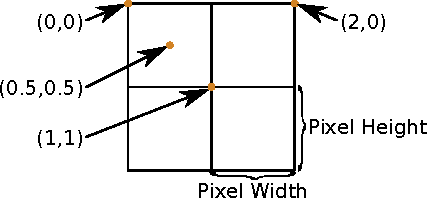
\includegraphics[width=0.8\textwidth]{pixel_coordinates.pdf}
\caption{Pixel coordinate system for a 2x2 pixels image.}
\label{fig:pixel_coordinates}
\end{figure}
}


\member{image\_size}{The width, height and depth of the image. For
  real space images this corresponds to the length and for reciprocal
  space ones to the inverse length of the sides of the image.}

\member{is\_fft\_shifted}{If set to 1 the image is assumed to have to
  the quadrants shifted (see Fig. \ref{fig:fft_shift}).

\begin{figure}[h!]
\centering
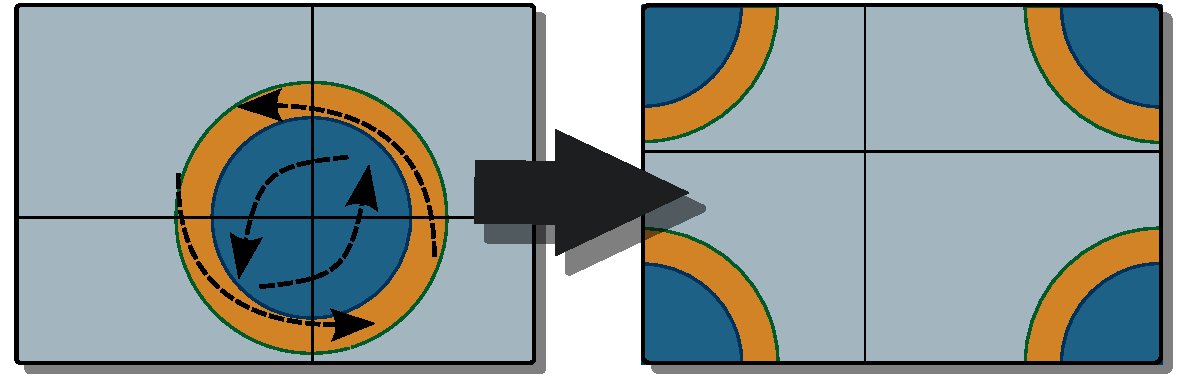
\includegraphics[width=0.8\textwidth]{fft_shift.pdf}
\caption{FFT shifting a 2 dimensional image.}
\label{fig:fft_shift}
\end{figure}
}

\member{mask}{32-bit mask specifying the properties of each
pixel.

The following list defines the meaning of each
bit when is it set, as well as the names of constants, defined in {\tt
cxi.h}, useful for
checkings their values:

\begin{table}[h!]\footnotesize
\caption{Definition of each bit in the mask}
\begin{tabular*}{\textwidth}{@{\extracolsep{\fill}} l p{5.5cm} l}
\toprule
\sf \bfseries Bit & \sf \bfseries Meaning & \sf \bfseries Constant \\
\midrule
\tt \bfseries 0x00000001 & \sf If set the pixel is valid & \tt
CXI\_PIXEL\_IS\_VALID\\
\tt \bfseries 0x00000002 & \sf If set the pixel is saturated & \tt
CXI\_PIXEL\_IS\_SATURATED\\
\tt \bfseries 0x00000004 & \sf If set the pixel is hot & \tt CXI\_PIXEL\_IS\_HOT\\
\tt \bfseries 0x00000008 & \sf If set the pixel is dead & \tt
CXI\_PIXEL\_IS\_DEAD\\
\tt \bfseries 0x00000010 & \sf If set the pixel is under a shadow &
\tt CXI\_PIXEL\_IS\_SHADOWED\\
\tt \bfseries 0x00000020 & \sf If set the pixel is iluminated by
parasitic light &
\tt CXI\_PIXEL\_IS\_PARASITIC\\
\tt \bfseries 0x00000040 & \sf If set the pixel signal is above the background &
\tt CXI\_PIXEL\_HAS\_SIGNAL\\
\bottomrule
\end{tabular*}
\end{table}

All other bits have no standard meaning and can be used for any
purpose the user sees fit. More bits will be defined as the format
evolves so users are encouranged to use the high bits to avoid collisions.}

\member{process\_$N$}{Processes used to obtain this image. They should
be listed in chronological order with the first processed used named
process\_1, the second process\_2 and so on.}

\member{reciprocal\_coordinates}{The diffraction (Fourier) space
  coordinates of the center of each pixel. Note that the dimension corresponding to
  the 3 different components should go before the image dimensions. So
  for example for an image of size [10,20,5] te reciprocal\_coordinates
will have size [3,10,20,5].}

\member{source\_$N$}{Link to the source used to obtain this image.}

\subsection{Instrument}
\label{table:instrument}

Template of instrument descriptions comprising various beamline
components. Each component will also be a class defined by its
distance from the sample. Negative distances represent beamline
components that are before the sample while positive distances
represent components that are after the sample. This device allows the
unique identification of beamline components in a way that is valid
for both reactor and pulsed instrumentation.

 Each Instrument instance
corresponds to one beamline.

\begin{table}[h!]\sffamily \footnotesize
\caption{Instrument class members}

\rowcolors{1}{white}{tableBlue}
\begin{tabular}{p{4.5cm} p{4.5cm}  p{2.5cm} }

\toprule
\bfseries Member     & \bfseries Type & \bfseries Quantity \\
\midrule

name & string & text \\
attenuator\_$N$ &  \hyperref[table:attenuator]{Attenuator class} & \\
detector\_$N$ &  \hyperref[table:detector]{Detector class} & \\
source\_$N$ &  \hyperref[table:source]{Source class} & \\
\bottomrule
\end{tabular}
\end{table}

\member{name}{Name of the instrument.}

\member{attenuator\_$N$}{The attenuators that are part of the
 instrument.}

\member{detector\_$N$}{The detectors that compose the instrument.}

\member{source\_$N$}{The source used by the instrument.}

\subsection{Note}
\label{table:note}

This class can be used to store additional information in a CXI file
e.g. additional text logs, configuration files, pictures, movies, audio.

\begin{table}[h!]\sffamily \footnotesize
\caption{Note class members}

\rowcolors{1}{white}{tableBlue}
\begin{tabular}{p{4.5cm} p{4.5cm}  p{2.5cm} }
\toprule
\bfseries Member     & \bfseries Type & \bfseries Quantity \\
\midrule

author & string & text \\
data & char array & binary/text \\
date & string & text \\
description & string & text \\
file\_name & string & text \\
type & string & text \\
\bottomrule
\end{tabular}
\end{table}

\member{author}{Author or creator of note.}

\member{data}{Binary/text note data.}

\member{date}{Date note created/added.}

\member{description}{Title of an image or other details of the note}

\member{file\_name}{Name of original file name if note was read from
 an external source.}

\member{type}{Mime content type of note data field e.g. image/jpeg,
 text/plain, text/html.}

\subsection{Orientation}
\label{table:orientation}

This is the description for a general orientation of a component - it
is used by the Geometry class.

\begin{table}[h!]\sffamily \footnotesize
\caption{Orientation class members}

\rowcolors{1}{white}{tableBlue}
\begin{tabular}{p{4.5cm} p{4.5cm}  p{2.5cm} }
\toprule
\bfseries Member     & \bfseries Type & \bfseries Quantity \\
\midrule

value & 6 floats & unitless \\
\bottomrule
\end{tabular}
\end{table}

\member{value}{Dot products between the local and the global unit vectors.}

The orientation information is stored as direction cosines. The
direction cosines will be between the local coordinate directions and
the global coordinate directions. The unit vectors in both the
local and global coordinates are right-handed and orthonormal. 

Calling the local unit vectors ($x',y',z'$) and the reference unit vectors
($x,y,z$) the six numbers will be [$x' \cdot x, x' \cdot y, x' \cdot z, y' \cdot
x, y'  \cdot y, y' \cdot z$] where "$\cdot$" is the scalar dot product (cosine
of the angle between the unit vectors). 

Notice that this correspods to the first two rows of the rotation
matrix that transforms from the global orientation to the local
orientation. The third row can be recovered by using the fact that the
basis vectors are orthonormal.

\subsection{Process}
\label{table:process}

Document an event of data processing, reconstruction, or analysis.

\begin{table}[h!]\sffamily \footnotesize
\caption{Process class members}

\rowcolors{1}{white}{tableBlue}
\begin{tabular}{p{4.5cm} p{4.5cm}  p{2.5cm} }
\toprule
\bfseries Member     & \bfseries Type & \bfseries Quantity \\
\midrule
command & string & text \\
comments & string & text \\
date & string & text \\
note\_$N$ &  \hyperref[table:note]{Note class} & \\
program & string & text \\
version & string & text \\
\bottomrule
\end{tabular}
\end{table}

\member{command}{Command line used to run the program.}

\member{comments}{Comments related to how the data was processed.}

\member{date}{Date and time of processing in ISO 8601 format.}

\member{note\_$N$}{Notes providing extra information like
  configuration files used, other inputs required or any other
  important information.}

\member{program}{Name of the program used.}

\member{version}{Version of the program used.}


\subsection{Sample}
\label{table:sample}

This class holds basic information about the kind of sample used, its
geometry and properties.

\begin{table}[h!]\sffamily \footnotesize
\caption{Sample class members}

\rowcolors{1}{white}{tableBlue}
\begin{tabular}{p{4.5cm} p{4.5cm}  p{2.5cm} }
\toprule
\bfseries Member     & \bfseries Type & \bfseries Quantity \\
\midrule
concentration & float & mass/volume \\
description & string & text \\
geometry\_1 &  \hyperref[table:geometry]{Geometry class} & \\
mass & float & mass \\
name & string & text \\
temperature     & float & temperature  \\
unit\_cell & 6 floats & length/angle \\
unit\_cell\_group & string & text \\
thickness & float & length \\
unit\_cell\_volume & float & volume \\
\bottomrule
\end{tabular}
\end{table}

\member{concentration}{Concentration of the sample.}

\member{description}{Description of the sample.}

\member{geometry\_1}{Position and orientation of the center of mass of the sample.}

\member{mass}{Mass of sample.}

\member{name}{Descriptive name of sample.}

\member{temperature}{Sample temperature.}

\member{unit\_cell}{Unit cell parameters (a,b,c
  $\alpha,\beta,\gamma$).}

\member{unit\_cell\_group}{Crystallographic space group of the crystal
  in PDB format.}

\member{thickness}{Sample thickness.}

\member{unit\_cell\_volume}{Volume of the unit cell.}


\subsection{Source}
\label{table:source}

Class describing the light source being used.

\begin{table}[h!]\sffamily \footnotesize
\caption{Source class members}

\rowcolors{1}{white}{tableBlue}
\begin{tabular}{p{4.5cm} p{4.5cm}  p{2.5cm} }
\toprule
\bfseries Member     & \bfseries Type & \bfseries Quantity \\
\midrule
energy     & float & energy  \\
pulse\_energy  & float & energy  \\
pulse\_width  & float & time  \\
\bottomrule
\end{tabular}
\end{table}

\member{energy}{Energy of each photon.}

\member{pulse\_energy}{Sum of the energy of all the photons in the pulse.}

\member{pulse\_width}{Duration of the pulse.}

\subsection{Translation}
\label{table:translation}

This is the description for the general spatial location of a component - it is used by the Geometry class

\begin{table}[h!]\sffamily \footnotesize
\caption{Translation class members}

\rowcolors{1}{white}{tableBlue}
\begin{tabular}{p{4.5cm} p{4.5cm}  p{2.5cm} }
\toprule
\bfseries Member     & \bfseries Type & \bfseries Quantity \\
\midrule

distances & 3 floats & length \\
\bottomrule
\end{tabular}
\end{table}

\member{distances}{The x, y and z components of the translation of the origin of the object
  relative to the origin of the global coordinate system (the place
  where the X-ray beam meets the sample).}
\normalsize

\clearpage
\section{Diagrams color code}
\label{color_code}

\begin{figure}[h!]
\centering
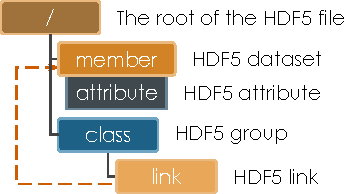
\includegraphics[width=0.6\textwidth]{diagram_labels.pdf}
\caption{Explanation of the color code used in the diagrams}
\label{fig:color_code}
\end{figure}

\clearpage
\section{Code examples}

All the code examples as well as the resulting CXI files are available from \url{cxidb.org}.
 
\subsection{Creating a minimal CXI file}
\lstset{
caption={Creating a minimal CXI file}
}
\lstinputlisting[language=Python]{minimal_cxi.py}
The resulting file should be equivalent to the one in
Fig. \ref{fig:minimal}.

\clearpage
\subsection{Creating a typical raw CXI file}
\lstset{
caption={Creating a typical raw CXI file}
}
\lstinputlisting[language=Python]{typical_raw_cxi.py}
The resulting file should be equivalent to the one in
Fig. \ref{fig:lcls_camp_raw}.

\clearpage
\subsection{NeXus compatible version of the typical raw CXI file}
\lstset{
caption={NeXus compatible version of the typical raw CXI file}
}
\lstinputlisting[language=Python]{nexus_cxi.py}
The resulting file should be equivalent to the one in
Fig. \ref{fig:lcls_camp_raw_nexus}.

\clearpage
\subsection{3D complex valued Image file}
\lstset{
caption={3D complex valued Image file}
}
\lstinputlisting[language=Python]{phased_3d_cxi.py}
The resulting file should be equivalent to the one in Fig. \ref{fig:phased_image}.

\clearpage
\subsection{Spartan viewer for CXI files}
\lstset{
caption={Spartan viewer for CXI files}
}
\lstinputlisting[language=Python]{spartan_cxi_viewer.py}
This simple program provides a way to view CXI files. Does not support
3D or complex valued data. To use it pass the name of the file
you which to view as a command line argument.
\end{document}